% !TeX spellcheck = en_US
\documentclass[journal,twoside]{IEEEtran}
\usepackage{graphicx}
\usepackage{url}
%\usepackage{slashbox}
\usepackage{cite}
\usepackage{amsmath}
\usepackage{enumerate}
%\usepackage{algorithm}
\usepackage{algorithmic}
\usepackage{multirow}
\usepackage{subfigure}
\usepackage{float}
\usepackage{booktabs}
\usepackage{epstopdf}
\usepackage{subfigure}
\usepackage{multicol}
\usepackage{txfonts}
\usepackage{bm}
\usepackage{supertabular}
\usepackage{xr}
\usepackage{makecell}
\usepackage{changepage}
\usepackage{threeparttable}
\usepackage{bbding}
\usepackage[linesnumbered,ruled,vlined]{algorithm2e}
\usepackage{graphicx} 
\usepackage{float}  
\usepackage{subfigure}  

%\usepackage{float}
%\usepackage{subfig}
%\usepackage{caption}
%\usepackage{subcaption}
%% \jvol{XX}
%% \jnum{XX}
%% \paper{1234567}
%% \pubyear{2020}
%% \publisheddate{xxxx 00, 0000}
%% \currentdate{xxxx 00, 0000}
%% \doiinfo{TQE.2020.Doi Number}

%\usepackage{slashbox}
%\usepackage{diagbox}
%\usepackage{tabularx}
\usepackage{color}
\definecolor{blue}{rgb}{0,0,1}

% correct bad hyphenation here
\hyphenation{op-tical net-works semi-conduc-tor}

\begin{document}
\title{Deep Learning-based Search Space Reconstruction Empowers Evolution Algorithm for Optimization}
\author{
    Yaotong Song,  Kaiyu Wang, Zhi-Hui Zhan,~\IEEEmembership{Fellow,~IEEE}, \\
    Zhenyu Lei, and Shangce Gao,~\IEEEmembership{Senior Member,~IEEE}  
    \thanks{\quad This research was partially supported by the Japan Society for the Promotion of Science (JSPS) KAKENHI under Grant JP23K24899, Japan Science and Technology Agency (JST) Support for Pioneering Research Initiated by the Next Generation (SPRING) under Grant JPMJSP2145, and the National Natural Science Foundation of China (Grant Nos. 62072483 and 62203238).}
    \thanks{\quad Y.~Song, K.~Wang, Z.~Lei and S.~Gao are with the Faculty of Engineering, University of Toyama, Toyama-shi, 930-8555, Japan. (E-mail: sytforwork@gmail.com; greskofairy@gmail.com; leizystu@outlook.com; gaosc@eng.u-toyama.ac.jp).}
	\thanks{\quad Z.~Zhan  is with the College of Artificial Intelligence, Nankai University, Tianjin 300350, China. (E-mail: zhanapollo@163.com).} 
}

\maketitle
% make the title area

\begin{abstract}
Evolutionary algorithms serve as a pivotal tool in addressing black-box problems, finding widespread applications across diverse academic disciplines and engineering domains. Despite their utility, these algorithms often confront challenges when navigating high-dimensional search spaces, impeding a comprehensive exploration of potential solutions. Relying solely on the algorithm's exploration capabilities proves insufficient for fully leveraging the information inherent in high-dimensional search spaces. To unlock the full potential of high-dimensional solution spaces, we introduce a deep learning method for the reconstruction of the search space. Specifically, discrete data sampled by evolutionary operators during the exploration process are collected, and a uniquely designed fully connected neural network is employed to reconstruct the exploration paths. The neural network's robust fitting capability facilitates the transformation of initially discrete sampled information into a continuous form. By capitalizing on the reconstructed solution space information, the algorithm excels in identifying superior solutions. We refer to this method of deep learning-based search space reconstruction evolution strategy algorithm (DLES). \textcolor{blue}{The effectiveness of DLES is validated across multiple datasets, including CEC 2014, CEC 2018, CEC 2022 and BBOB. Experimental results, compared to several state-of-the-art algorithms, affirm the superiority of the DLES algorithm.}
\end{abstract}

\begin{IEEEkeywords}
	Evolutionary computation, deep learning, search space reconstruction, artificial neural network, single-objective optimization.
\end{IEEEkeywords}

\IEEEpeerreviewmaketitle

\section{Introduction}
\IEEEPARstart{E}{volutionary} computation (EC) is a powerful tool to address complex optimization problems \cite{eiben2015evolutionary}. Inspired by biological evolution, evolutionary algorithms assess the fitness of real-valued solutions to promote the progress of search. The best solution vectors are retained while other solutions that are not favorable to evolution are discarded. The surviving high-quality solutions are subsequently subjected to crossover and mutation to generate the next generation. This crossover approach addresses the limitations of traditional algorithms that have massive variables and are prone to prolonged convergence, making them difficult to train \cite{li2023machine}.

The primary goal of EC is to optimize a given objective function and identify the optimal solution within defined constraints \cite{Shangcegao2019chaotic}. Nevertheless, when dealing with extensive representational data like images and text, EC approaches often face limitations and overpower. Therefore, deep learning (DL) was introduced to tackle these daunting tasks in the early 21st century. DL has witnessed remarkable success, particularly in computer vision, natural language processing, image and speech recognition, etc \cite{Boiko2023}. Deep neural networks are trained to automatically update connection weights to achieve better learning results and handle tasks more effectively \cite{lee2022complex}. The rapid advancement of DL is driven by factors such as large-scale datasets, enhanced hardware capabilities, and improved algorithms, positioning it as a key driving force in the field of artificial intelligence \cite{9552976, ma2023estimating}.

Although EC and DL have different tasks and goals, the interplay between the two branches has been a subject of keen scholarly interest. A superior DL model can automatically fine-tune neural network weights and parameters to achieve desired outcomes. Meanwhile, EC is geared toward exploring solution spaces to discover optimal solutions without an inherent learning process \cite{lei2023chaotic}. Borrowing EC to evolve the topology of neural networks or using neural networks to empower learning capabilities within EC are exciting sources of inspiration. Therefore, researchers have aimed to unify EC and DL to harmonize and complement each other to generate a more powerful artificial intelligence tool \cite{yu2021improving}.

Neuroevolution stands out as a successful approach to optimizing artificial neural networks among so many combinatorial attempts. It utilizes evolutionary algorithms or some EC techniques to train various aspects of neural networks, including activation functions, hyperparameters, neural architectures, etc. Initially, researchers endeavor to investigate whether evolutionary algorithms could replace backpropagation to evolve a network's weights and hyperparameters \cite{galvan2021neuroevolution}. Configuring reasonable hyperparameters faces difficulties such as different types of variables, large search scale space, and high evaluation costs. To address these challenges for convolutional neural networks, Li et al. \cite{9540902} propose a novel hybrid distribution estimation algorithm. This algorithm employs hybrid variable hyperparameters encoding coupled with an orthogonal initialization strategy, effectively managing the extensive search space. Notably, it excels in hyperparameter optimization, as evidenced by its robust performance in medical diagnostics. Owing to the conclusion that evolutionary methods can be effectively applied to optimize network topology and connection weights, scholars challenge whether reasonable neural architectures can be searched directly with evolutionary algorithms. The process of constructing a suitable target architecture requires a great deal of experimentation and trial-and-error due to the multitude of structural variables and the significant computational overhead. Neural architecture search can effectively jump out of the inherent thinking paradigm and allow algorithms to compute complex and effective topologies automatically. Chen et al. \cite{chen2019renas} integrate reinforcement mutation strategies into neural architecture search, steering the efficient evolution of populations in the model to evolve to a better state with fewer computational resources. The reinforced evolutionary neural architecture search achieves competitive accuracy and semantic segmentation performance on multiple extensive datasets.

The integration of evolutionary algorithms with neural networks has been validated through various examples, demonstrating their ability to support or even execute neural network functions and tasks effectively. In recent years, scholars have been keen to imbue evolutionary populations with the concept of learning ability. Nevertheless, most attempts to incorporate learning models into evolutionary algorithms have performed poorly, hindered by the dual black-box nature of neural networks and optimization processes. This impasse is broken with the emergence of transfer learning, which adeptly introduces a learning dimension into EC \cite{zhang2023survey}. Transfer learning leverages knowledge gained from one problem to expedite solutions to related issues, transferring insights based on function evaluation outcomes to either homogeneous or heterogeneous search spaces. In a parallel vein, reinforcement learning, with its exploratory approach, augments the search prowess of evolutionary algorithms through iterative trial and error. These concepts of learning and paradigms of problem-solving exhibit remarkable compatibility when integrated into the algorithmic processes of solving, searching, and evolving.

The integration of evolutionary algorithms with neural networks collectively represents a burgeoning field, poised to mitigate inherent limitations in both domains. This synergy heralds a promising trajectory for the refinement of evolutionary algorithm exploration and exploitation, as well as the enhancement of neural networks. The predominant emphasis in current research on the integration of evolutionary algorithms and deep learning is the optimization of algorithmic hyperparameters. Additionally, some studies concentrate on leveraging surrogate models to emulate abstract search spaces \cite{he2023review}, facilitating effective exploration within broader search domains. This emphasis contributes to the improved sampling efficiency of algorithms within the expansive search space. There is a noticeable lack of attention directed towards modeling the authentic search space to extract greater solutions. Hence, we investigate the feasibility and impact of the network in reconstructing the authentic solution space on the population.
\begin{figure}[t]
	\centering
	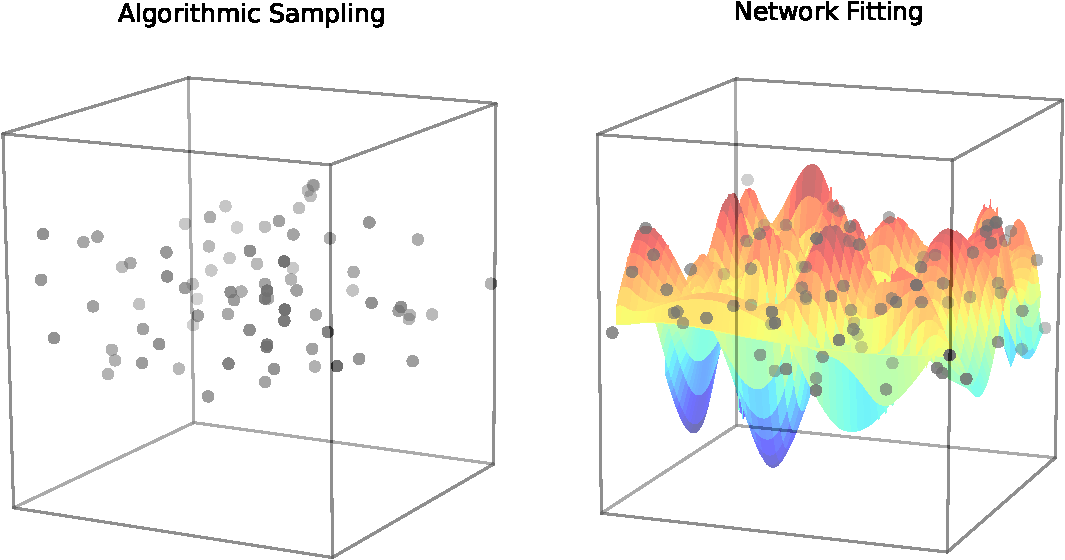
\includegraphics[width=0.4\textwidth]{./net_fitting.pdf}
	\caption{Visualization of algorithm sampling and network reconstruction.}
	\label{net_fitting}
\end{figure}

Fig.~\ref{net_fitting} provides a visual representation of utilizing a neural network to reconstruct the search space based on the sampling results of evolutionary operators within the authentic search space, aiming to obtain higher-quality solutions. The points in the figure represent the sampling results of the algorithm in the search space. The results of the network reconstruction are shown on the right side of the figure, with colors ranging from red to blue. The bluer color denotes the higher quality of solutions. While the algorithm samples discretely within the search space, the results by network reconstruction become continuous. Observably, the network demonstrates the capability to discern solutions of superior quality within the search space through the reconstruction of algorithmically sampled results. In this paper, we propose a deep learning-based search space reconstruction evolution strategy algorithm (DLES) that harnesses the formidable fitting capabilities of neural networks to reconstruct the authentic search space, thereby enhancing the quality of the solution. Distinguishing itself from other methods that incorporate neural networks in EC, our approach acquires superior individuals directly from the network based on its reconstruction results to the search space. To the best of our knowledge, we are the first to employ deep learning for reconstructing the authentic search space. The main contributions of this work include the following:
\begin{itemize}
	\item[1)] Innovatively, we propose a novel DLES algorithm, it employs a novel full-connected neural network to reconstruct the search space. The network utilizes the fitness as its input to construct individual information as the output. It is noteworthy that the input dimension of the network is set to one, deviating significantly from conventional network architectures.	
	
	\item[2)] Initially, we design the neural network to address a discrete sample of solution space. It vastly extends the sample, making the algorithm gain a more nuanced understanding of the search space, thereby assisting in the discovery of superior solutions.

	
	\item[3)] We perform massive experiments to verify the performance of DLES on diverse CEC test sets, compared with state-of-the-art algorithms, which demonstrate DLES's superiority. Besides, we comprehensively analyze the impact of hyperparameters and space reconstruction networks to achieve stable and robust performance. 
	
	
\end{itemize} 

Section~\ref{prelim} gives a preliminary about the evolution strategy and the related work of learning evolutionary computation. Section~\ref{methods} details the DLES. Section~\ref{Expre and analy} illustrates the experiments with results and analyses. Finally, the conclusion is provided in Section~\ref{sec_conclusion}.


\section{Preliminaries}\label{prelim}
This section introduces the evolution strategy and the related work of learning evolutionary computation.

\textcolor{blue}{
\subsection{Evolutionary Computation}
EC is an essential tool in the field of optimization, known for their ability to solve complex and nonlinear problems that are often beyond the reach of traditional optimization methods. EC is inspired by the principles of natural evolution and includes a variety of algorithms such as genetic algorithm, evolution strategies, differential evolution, etc. These algorithms are designed to mimic the process of natural selection, where a population of candidate solutions evolves over time, guided by fitness functions that measure the quality of solutions. Through mechanisms like selection, crossover, and operators, evolutionary algorithms explore the solution space and converge towards optimal or near-optimal solutions.}

\textcolor{blue}{
Evolutionary algorithms also, represent a broader class of optimization techniques, which are designed to provide high-quality solutions to complex problems by combining heuristic methods with strategies for escaping local optima, thus balancing exploration and exploitation of the search space \cite{10630664}. They are particularly effective for problems where the search space is vast, rugged, or poorly understood, making them versatile tools for a wide range of applications.}

\textcolor{blue}{
Evolutionary algorithms have been successfully applied to various domains, including engineering design, logistics, scheduling, machine learning, and bioinformatics. Their ability to handle complex, multi-objective, and dynamic optimization problems has made them a popular choice among researchers and practitioners \cite{li2023survey}. However, the design and implementation of effective metaheuristic algorithms require a deep understanding of both the problem domain and the algorithm's behavior, as well as careful tuning of parameters to achieve the best performance.}

\textcolor{blue}{
In conclusion, evolutionary algorithms provide a powerful and versatile tool for solving complex optimization problems. Their ability to find good solutions in challenging search spaces makes them invaluable in a wide range of applications. However, the successful application depends on a careful balance of exploration and exploitation, proper parameter tuning, and, in some cases, the integration of problem-specific knowledge to enhance performance.}

\subsection{Evolution Strategy}
Evolutionary strategy (ES) is a heuristic technique for black-box optimization, widely applied across various disciplines and engineering domains \cite{10324315,10265195}. The ES aims to simultaneously generate solution vectors with the advantage of fewer evaluations and computational resources. The design principles of ES are unbiasedness, randomization, and adaptive control over samples \cite{10056413}. The most widely used is the covariance matrix adaptation evolution strategy (CMAES) due to its rotational invariance, making it effective for targeting unimodal continuous optimization problems \cite{hansen2001completely}. CMAES obtains the covariance matrix $\mathcal{C}$ through matrix decomposition and transformation in the search space, aiding in making the objective function separable for efficient solving. CMAES updates the covariance matrix by evolving the weighted maximum likelihood estimates for the selected directions. This updating process can be expressed as \cite{karmakar2023cma}:
\begin{equation}
	\mathcal{C}_{g+1} = (1 - c_1 - c_c)C_g + c_1P_{g+1}P^T_{g+1}+c_c\sum_{i = 1}^\lambda\Gamma_i,
\end{equation}
where $g$ denotes the number of iterations; $c_1$ and $c_c$ represent the scale transformation rates of the covariance matrix; $\lambda$ is the number of promising individuals in the top $\lambda$ rankings. $P$ is called the evolutionary path and denotes the accumulation of the mean of the historical distribution. $\Gamma_i$ denotes the mutation according to the Gaussian variational distribution for the $i$th individual. The original CMAES faces challenges of computational expense and sensitivity to boundary constraints. Moreover, its covariance matrix struggles to capture variable relationships in multimodal search spaces \cite{li2020variable}. Numerous variants have emerged to address these issues, with the hybrid sampling evolution strategy (HSES) standing out as the CEC 2018 winner \cite{zhang2018hybrid}. HSES introduces a hybrid sampling strategy that mitigates CMAES limitations by leveraging the robustness of univariate sampling in handling multimodal problems.

Another popular approach is the family of natural evolution strategies (NES). This family encompasses a group of gradient estimation algorithms associated with specific types of distributions. NES involves evaluating the fitness function at each sample point and computing gradients in the direction of higher expectations. Natural gradients excel in overcoming challenges like unstable performance and premature convergence. Wierstra et al. \cite{wierstra2014natural} explore NES and discover that the enhanced NES exhibits strong parallelism, excellent data processing efficiency, and effective exploration.

\textcolor{blue}{
To conclude, ES focuses on mutation and operations and generally does not employ crossover operation, making the optimization process more stable, particularly when addressing multimodal or high-dimensional problems. Since ES does not depend on population recombination, it is less sensitive to the choice of the initial population, exhibiting strong robustness. Even with a low-quality initial solution, the algorithm can gradually converge to an optimal solution. ES is inherently designed for continuous optimization problems in high-dimensional spaces, especially those involving noise, nonlinearity, or complex multimodal landscapes. Given these advantages, we utilize evolution strategies, a fundamental EC method, to explore the solution space without introducing other complex mechanisms.
}

\subsection{Learning-based Evolutionary Computation}
In recent years, the challenges of incorporating learning abilities into evolution algorithms have been steadily addressed with the emergence of various learning models and the advancements in neural networks. Scholars have actively explored ways to integrate and enhance neural networks across various aspects of algorithmic structures, operators, and search patterns, resulting in significant successes. Currently, there are two main directions for modifying evolutionary algorithms through learning. The first direction involves employing learning models, such as transfer learning and reinforcement learning. These bio-inspired learning models naturally align with different processes of EC, effectively enhancing the optimization and generalization capabilities of the algorithms \cite{yangyuDE2018}. The second involves directly embedding neural networks into the evolutionary search process. This integration assists the evolutionary population in decision-making, optimization, learning, and other operations. This dual approach reflects the ongoing efforts to synergize evolutionary algorithms with the power of learning models, marking a promising advancement in the field.

Evolutionary transfer optimization has emerged as a promising approach in the EC community \cite{9321762}. This method involves transferring knowledge, such as population trajectories and individual information, from a historical task or an ongoing optimization task to address relevant new problems. This cross-domain transfer learning approach has been successful in complex optimization and has developed branches such as sequential optimization, multi-task optimization, etc. Jiang et al. \cite{9097186} propose a novel algorithmic framework that integrates streaming transfer learning and memory mechanisms. By leveraging historical experience, this framework enables the population to learn the optimal potential space, significantly enhancing optimization speed without compromising solution quality. Qiao et al. \cite{qiao2023evolutionary} develop an evolutionary multi-task model to solve constrained multi-objective problems. The model establishes three tasks, namely the main search task, the global auxiliary task, and the local auxiliary task, facilitating efficient population search through the transfer of information between different tasks.

With the successful application of transfer learning in optimization, the integration of reinforcement learning into the EC framework has aroused enthusiasm, resulting in numerous reinforcement learning-assisted evolutionary algorithms. A distinctive feature of reinforcement learning is its utilization of an agent learning process grounded in Markovian decision-making for maximizing rewards \cite{10172347}. The integrated approach generally determines the states, actions, and rewards in the decision chain based on the design goals of the algorithm and acts as an auxiliary regulator of the algorithm's search strategy. Sun et al. \cite{sun2021learning} innovatively incorporate a deep neural network as a controller for control parameters, coupling it with a reinforcement policy gradient algorithm to optimize the best parameters. This approach dynamically provides optimal parameter settings tailored to match the characteristics of test functions. Zhang et al. \cite{10035716} propose a hybrid adaptive parameter control framework employing Q-learning and deep Q-learning to regulate agents. This self-switching learning model significantly enhances the solution quality of the original algorithm, verifying that empowering the algorithm to learn is a catalyst for optimization. Chrabaszcz et al. \cite{chrabaszcz2018back} demonstrate that ES serves as a viable alternative to reinforcement learning algorithms in addressing a range of challenging deep reinforcement learning problems.

In addition to the previous embedding of learning models, neural networks have been directly involved as trainers in EC in recent years. Ismayilov and Topcuoglu \cite{ismayilov2020neural} propose a dynamic multi-objective optimization algorithm based on artificial neural networks, showcasing effective performance on dynamic workflow scheduling problems. This algorithm utilizes a multi-layer neural network to train paired solutions output, thereby grasping high-quality solutions. Zhan et al. \cite{10002945} introduce a network-assisted learning-evolutionary algorithm, providing the evolutionary operator with the ability to learn and generate promising next-generation individuals. This learning operator learns from numerous successful solutions and training to enhance the entire evolutionary search process. Despite the challenges posed by neural networks simulating the intricate situation of black-box optimization and the trajectory of evolutionary populations, the training and learning results often show some limitations. There remains significant potential to explore in this direction, and maximizing the benefits of neural networks in evolutionary computation presents a compelling and intriguing topic.

\section{The proposed methods}\label{methods}
The section describes the motivation and the details of DLES. The proposed DLES reconstructs the authentic search space with a deep learning network, enhancing the algorithm's capability to navigate high-dimensional search spaces. This assists the algorithm in locating more optimal solutions.  

\subsection{Motivation}
% Evolutionary algorithms and neural networks are two formidable tools for addressing black box problems, each possessing unique strengths. Combining these two methods allows for more significant advantages in dealing with complex problems, enabling a deeper understanding of the structure of high-dimensional search spaces \cite{10068274}.
\textcolor{blue}{
Evolutionary algorithms and neural networks are powerful tools for solving black-box problems. Combining them leverages their strengths to better handle complex problems and gain deeper insights into high-dimensional search spaces \cite{10068274}.}
%The complexity of high-dimensional search spaces presents a significant challenge, making comprehensive simulation directly impractical. The surrogate-assisted evolutionary method~\cite{he2023review} for dimensionality reduction simulations faces certain challenges in capturing all features of high-dimensional spaces \cite{9754323}. Additionally, it demands a significant consumption of computational resources, rendering it particularly expensive, which is more suitable for addressing the issue of costliness \cite{9542966}. Therefore, a more practical approach involves initially partitioning the solution space \cite{liu2023decision,9428697} and selectively addressing the crucial regions within it.

\textcolor{blue}{
High-dimensional search spaces pose a major challenge, making direct simulation impractical. Surrogate-assisted evolutionary methods for dimensionality reduction face difficulties in capturing all features of high-dimensional spaces and require substantial computational resources, making them costly \cite{9754323, he2023review, 9542966}. A more practical approach is to partition the solution space first and focus on selectively addressing key regions within it \cite{liu2023decision, 9428697}. }

%In the process of searching for the optimal individual within the search space, evolutionary algorithms primarily involve two stages: exploration and exploitation \cite{9272701}. The effectiveness of the exploration phase significantly influences the success of subsequent exploitation stages. Evolutionary algorithms sample the search space to understand its structure, but the discrete nature of sampling results makes it challenging to form a complete and accurate description. This limitation may cause the algorithm to overlook valuable exploration areas, leading to the trap of local optima.
\textcolor{blue}{
During the search for the optimal individual, evolutionary algorithms follow two main stages: exploration and exploitation \cite{9272701}. The success of the exploration phase is crucial for the effectiveness of the subsequent exploitation. While evolutionary algorithms sample the search space to infer its structure, the discrete nature of the sampling process makes it difficult to obtain a complete and accurate representation. This limitation may cause the algorithm to miss valuable areas and become trapped in local optima.}

\textcolor{blue}{
To address this challenge, we propose the DLES, leveraging the powerful non-linear fitting capability of neural networks to reconstruct these exploration paths. Exploration paths are the sequences of sampled points generated by the algorithm as it explores the solution space. By reconstructing these paths, DLES captures and utilizes the valuable information embedded within the exploration process. While the algorithm explores the solution space extensively, the exploration path occupies a significantly smaller portion compared to the full space. By focusing on reconstructing the exploration path, we substantially reduce the workload for network reconstruction, enabling us to complete the task with less complex networks. The goal is to discover high-quality areas overlooked by the algorithm due to insufficient exploration. By reconstructing the paths, we can achieve a more effective fit for authentic high-dimensional search spaces, providing the algorithm with a better potential area and reducing the risk of falling into local optima \cite{zhou2024evolutionary}.}
\begin{figure}[t]
	\centering
	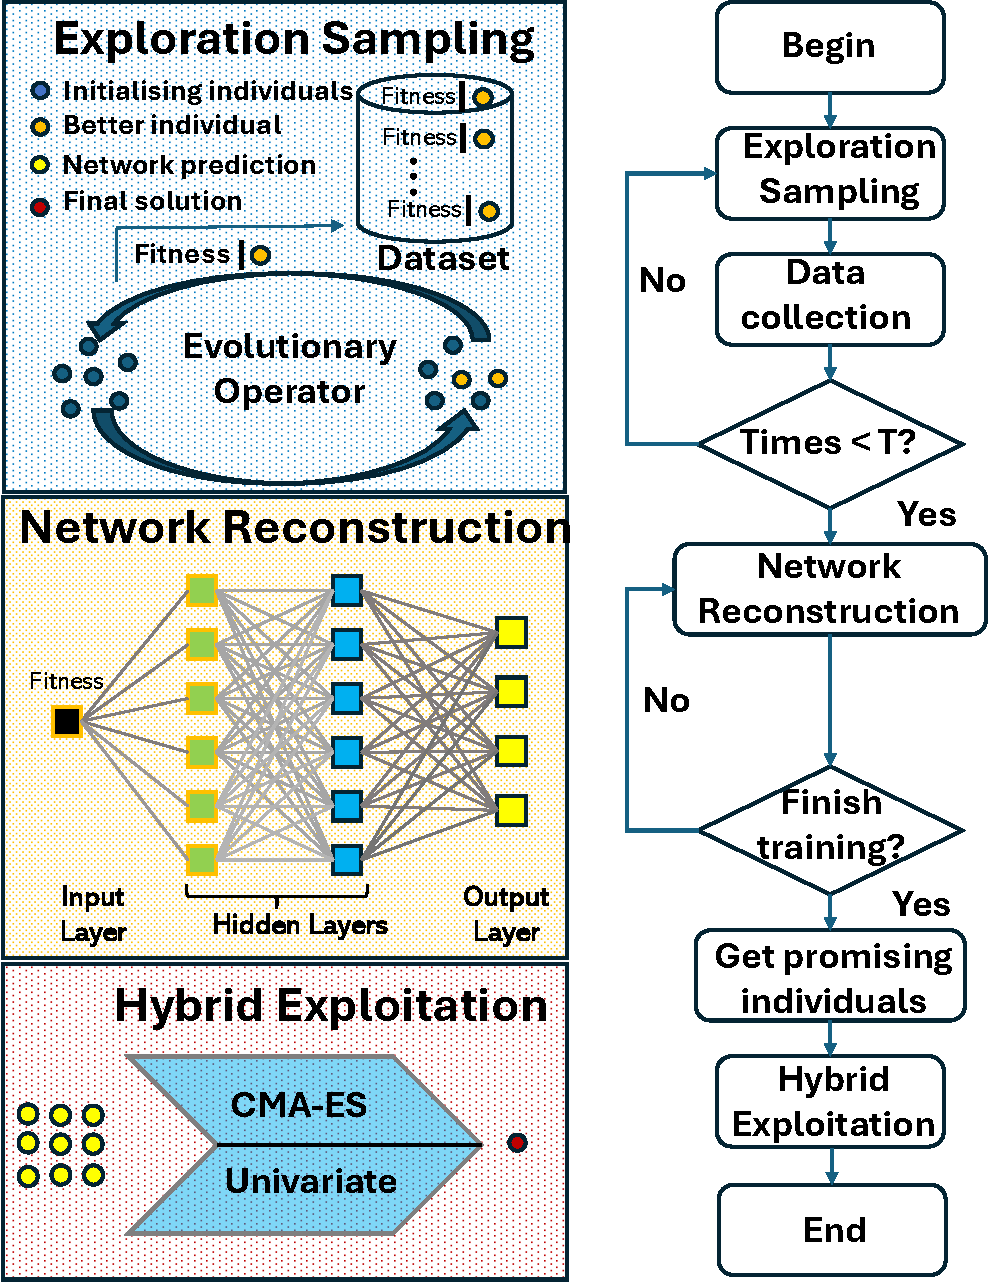
\includegraphics[width=0.9\columnwidth]{./struct.pdf}
	\vspace{-1mm}
	\caption{\textcolor{blue}{The structure and flow framework of DLES.}}
	\label{dles}
	\vspace{-2mm}
\end{figure}
\textcolor{blue}{
\subsection{Deep Learning-based Search Space Reconstruction Evolution Strategy}}
Building upon the concept of deep learning-based search space reconstruction empowers evolution algorithms for optimization, we introduce DLES. The overall structure and flow framework of DLES is depicted in Fig.~\ref{dles}. \textcolor{blue}{These components are executed in a sequential manner, comprising three distinct phases. The first phase, the evolutionary operator for exploration, explores the solution space and performs data collection and processing. In the subsequent phase, network reconstruction, the collected data is employed to reconstruct the solution space, thus facilitating the identification of more promising solutions for further exploration. The final phase, hybrid sampling for exploitation, leverages the network-generated solutions to execute the final optimization process.}

\subsubsection{Exploration Sampling}
The primary focus of this stage involves conducting a thorough exploration of the search space using an evolutionary operator sampling and systematically collecting a dataset. The goal is to facilitate comprehensive exploration by the algorithm, capturing a diverse set of highly representative data points to construct a dataset suitable for network learning. This approach ensures the effective reconstruction of the search space.
\subsubsection{Network Reconstruction}
After collecting a feasible dataset, a neural network reconstructs the authentic search space, revealing solutions with higher potential. The network extensively leverages the exploration of sampled datasets for profound learning and fitting. Upon concluding the reconstruction process, the network can generate solutions with elevated exploitation possibilities rooted in the collected dataset.
\subsubsection{Hybrid Exploitation}
As the final stage of the DLES, a hybrid sampling strategy is employed to exploit the solutions generated in the network predictions. This method amalgamates the benefits of both single-sampling and multi-sampling, augmenting search efficiency and result accuracy.


\subsection{Exploration Sampling}
In the exploration section, DLES utilizes traditional evolutionary operators, exploring the search space through sampling and gathering pertinent information to construct a dataset suitable for neural network learning.

First, define the evaluation function $F(\cdot)$ based on a optimization problem, initialize the population $P^{0}$, and set the current ($N\!F\!E\!s = 0$). During the exploration process, the population undergoes a cumulative total of $T$ iterations. The population $P^{t}$ at generation $t$ comprises $N$ individuals, each denoted as $y_{i}^{t}$, and each individual has a dimension of $D$. DLES employs an evolutionary operator $\rho(\cdot)$ to generate $M$ new individuals, forming the candidate set $P^{t'}$. Evaluating all candidates in $P^{t'}$ costs the evaluation function $F(P^{t'})$ to obtain the fitness values $\mathcal{F}$. Based on the fitness values, $N$ individuals are selected from $P^{t'}$ to constitute the new population $P^{t+1}$. By continually updating the population through the utilization of evolutionary operators, DLES samples within the solution space and then comprehensively explores it. Simultaneously, it gathers relevant information, forming a $Dataset$ conducive to neural network learning. 

Due to the intrinsic characteristics of evolutionary operators in the sampling process, the algorithm iteratively endeavors to optimize specific locations for the discovery of improved solutions. However, this iterative procedure may lead to generating a substantial amount of redundant information. \textcolor{blue}{To enhance the efficiency and effectiveness of network reconstruction, DLES records the information of the current best individual ($y_{best}$) and its corresponding fitness value ($f_{best}$) upon detecting a decrease in fitness. This means that the algorithm updates its records only when a superior solution is identified compared to the previous best. By doing so, DLES ensures that it consistently retains the most optimal solution encountered throughout the search process.} This information forms a dataset available for network learning. This decision avoids introducing excessive redundant information, ensuring that the neural network not only learns valuable information but fits the exploration path well. Throughout this process, the operators persistently attempt, make errors, and learn, progressively accumulating an understanding of the solution space. Such iterative procedures contribute to the stepwise optimization of the population, providing valuable learning $Dataset$ for the neural network.

\textcolor{blue}{
In DLES, an optimized univariate marginal distribution algorithm continuous (UMDAc) \cite{10247259} is chosen as the evolutionary operator $\rho(\cdot)$. UMDAc exhibits high computational efficiency and operates with minimal interactions between variables. By sampling from the learned marginal distributions, UMDAc effectively balances exploration and exploitation, facilitating a thorough exploration of the search space. This balance is crucial for ensuring comprehensive coverage within the solution space. Additionally, UMDAc demonstrates robustness to noise and varying problem conditions, enhancing its effectiveness across diverse optimization scenarios \cite{8790358}.}

This particular optimized UMDAc increases the weight of the best individual $y_{best}$ when computing the mean $\mu$. $\mu_{d}$ is to set the weighted sum of the best $N$ solutions on each variable $x_{d}$,
\begin{equation}
	\mu_{d} = \sum_{n=1}^{N} \omega_{n}x_{dn}.
\end{equation}
The weight $\omega_{n}$ are determined by following equations:
\begin{equation}
	\begin{aligned}
		\omega'_{n} = \ln(N + &0.5)-\ln(n), \quad n \in [1, N] \\
	\end{aligned}
\end{equation}
\begin{equation}
	\begin{aligned}
		\omega_{n} &= \frac{\omega'_{n}}{\sum_{n = 1}^N \omega'_{n}}.
	\end{aligned}
\end{equation}
The exploration pseudocode is presented in Algorithm~\ref{exploration}.

\begin{algorithm}[t]
	\caption{\textcolor{blue}{Exploration Sampling}} 
	\label{exploration} 
	\renewcommand{\algorithmicrequire}{\textbf{Input:}}
	\renewcommand{\algorithmicensure}{\textbf{Output:}}
	\begin{algorithmic}[1]
		\REQUIRE Initialization: $P^{0} \sim \mathcal{U}$, $P^{0} \in R^{d \times N}$, $Dataset$ = $\emptyset$, $N\!F\!E\!s = 0$, an evaluation function $F(\cdot)$ and an optimization function $\rho(\cdot)$
		\ENSURE $Dataset$ and $N\!F\!E\!s$
		%\STATE $\Gamma^{0} \leftarrow P^{0}$; // parameters for the $\rho(\cdot)$;
		\STATE $\mathcal{F} \leftarrow F(P^{0})$; 
		\STATE select $f_{best}$ from $\mathcal{F}$;
		\STATE $N\!F\!E\!s += N$;
		\STATE select $y_{best}$ from $P^{0}$ by $f_{best}$; //optimal individual 
		\STATE Add ($y_{best}$, $f_{best}$) in $Dataset$;
		\FOR{$t$ \textbf{from} 0 \textbf{to} $T$}
		\STATE $P^{t'}$ = $\rho(P^{t})$, $P^{t'} \in R^{d \times M}, N<M$;
		\STATE get $y_{best}^{t}$ , $f_{best}^{t}$ and $P^{t+1}$ from sorted $P^{t'}$\\ 
		$P^{t+1} = {P^{t'}_{i} \mid i \in [1, N]}$;
		\STATE	$N\!F\!E\!s += N$;
		\IF {$f_{best}^{t} < f_{best}$}
		\STATE	Add ($y^{t}_{best}$, $f^{t}_{best}$) in $Dataset$;
		\STATE  $f_{best}$ = $f_{best}^{t}$;
		\ENDIF	
		\ENDFOR
	\end{algorithmic} 
\end{algorithm}

\subsection{Network Reconstruction}
In the network reconstruction, a neural network utilizes data collected during the exploration process to reconstruct the authentic search space. Specifically, by learning from the sampled outcomes of evolutionary algorithms, neural networks can more directly and efficiently comprehend the structure of the search space. This capability enables neural networks to discover individuals situated along the exploration path, those that conventional evolutionary algorithms might overlook. These individuals exhibit greater exploitation potential.

In this research, we employ neural networks to reconstruct the paths in the search space by reverse deducing fitness value $f$, thereby providing an individual ($y$) with enhanced developmental potential. Specifically, the neural network takes $f$ as input and predicts individual information ($\hat{y}$) in a $D$-dimensional space. The network comprises three fully connected layers, it is formulated as follows:
\begin{equation}
	\begin{split}
		&net^{(in)} = W^{(in)} f + b^{(in)} \\
		&net^{(h)} = tanh(W^{(h)} net^{(in)} + b^{(h)})\\
		&net^{(out)} = W^{(out)} net^{(h)} + b^{(out)}, \\
	\end{split}
\end{equation}
where $W$ and $b$ represent the weights and bias of networks, respectively. $net^{(in)}$, $net^{(h)}$, and $ net^{(out)}$ represents the output of the input, hidden, and output layer. Notably, the network may include a different number of hidden layers. In hidden layers, the hyperbolic tangent function ($tanh$) is employed as the activation function,
\begin{equation}
	tanh(x) = \frac{e^{x}- e^{-x}}{e^{x} + e^{-x}}.
\end{equation}
This function excels at handling negative data, producing output within the range of $[-1, 1]$. This characteristic makes it approach linearity near the zero point, contributing to mitigating the issue of gradient vanishing. The input layer has a size of 1, the output layer has a size of $D$. Through hidden layers, the neural network maps the input fitness value to a high-dimensional space and then projects the high-dimensional results back to the corresponding $D$-dimensional space.

During the training phase, the neural network optimizes the weight matrices and bias terms to minimize the difference between ($\hat{y}$) and $y$ by the loss function. After training completion, the neural network, by fitting the information of the search space, can predict individual information corresponding to the input fitness value. When provided $y$ with the smaller fitness minimum one, the neural network's task is to offer individuals with greater potential based on the reconstructed search space information.

Regarding the loss function, mean squared error (MSE) is generally considered a reasonable option. However, we observed that network reconstruction faces significant challenges when relying on MSE. In the context of fitting with the MSE loss function, the loss in a network arises from the mean square error between the network predictions and the actual labels. This implies that the network assigns equal importance to all data points, leading to significant consumption of computational resources and frequently failing to attain an optimal fit. During the process of training the network for reconstruction, our expectation is for the network to focus on regions with better fitness quality while minimizing attention to areas with poor solution quality. Therefore, we adopt a newly designed fitness mean squared error (FMSE) loss function, the formula for which is presented below:
\begin{equation}
	\label{Eloss}
	loss = \frac{1}{D} \sum_{{i} = 1}^{D} \left|y_{i} - \hat{y_{i}}\right|^{2} + 
	{D} \frac{\left|f_{i} - f_{mean}\right|}{f_{std}}.
\end{equation}

\textcolor{blue}{
Due to the difference in units between the MSE and fitness components, there is a risk that the network may overlook the MSE part when the fitness values are excessively large. To address this, we normalize the fitness values to follow a normal distribution. To further ensure consistency between the two components and prevent significant numerical discrepancies, we multiply the normalized fitness values by the dimension $D$, thereby aligning the units of both components.}

The FMSE incorporates fitness into the computation, directing the network's attention toward regions with higher solution quality. By assigning lower loss values to regions with higher qualitative, the FMSE encourages the network to engage in more refined learning and optimization in these areas. The adoption of the FMSE allows the network to focus more on solution spaces with elevated fitness, thereby enhancing reconstruction performance and reducing computational resource consumption. This approach provides a novel pathway for achieving more efficient network training and better fitting within solution spaces. The network reconstruction pseudocode is presented in Algorithm~\ref{netwrok}.
\begin{algorithm}[t]
	\caption{Network Reconstruction} 
	\label{netwrok} 
	\renewcommand{\algorithmicrequire}{\textbf{Input:}}
	\renewcommand{\algorithmicensure}{\textbf{Output:}}
	\begin{algorithmic}[1]
		\REQUIRE $Dataset$, $f_{best}$
		\ENSURE A network-fitted optimal solution $y^{*}$
		\STATE Randomly initialize network parameters;
		\FOR{$e$ \textbf{from} 0 \textbf{to} $Epoch$}
		\FOR { pair in $Dataset$}
		\STATE  $f, y \leftarrow $ pair;  
		\STATE $\hat{y}$ = network($f$); 
		\STATE calculate $loss$ by (\ref{Eloss});
		\STATE update the network's parameters by $loss$;
		\ENDFOR
		\ENDFOR
		\STATE $y^{*}$ = network($f_{best}$);
	\end{algorithmic} 
\end{algorithm}

\subsection{Hybrid Exploitation}
In the exploitation section, we adopt a hybrid sampling approach using CMAES combined with univariate sampling \cite{8790358}. CMAES is particularly suitable for addressing unimodal problems, while single sampling is effective for handling multimodal problems. This combination combines multivariate sampling with univariate sampling to effectively enhance the algorithm's search performance across a wide range of problem types. Initially, CMAES is utilized to optimize the network-fitted optimal solution $y^{*}$, if multiple updates with CMAES yield no improvement in solutions, the execution of CMAES ceases and we obtain the optimal solution $y'$. Subsequently, $y'$ is ues to generate a new population, subsequently passed to univariate sampling for additional optimization. For univariate sampling, the population updates by the mean ($\mu_{d}$) and variance ($\sigma_{d}$) for each dimension. In order to guarantee the convergence of the algorithm, we set the parameter $cc$ to control the $\sigma_{d}$, with $cc$ approaching but remaining below 1 ($cc \rightarrow 1^{-}$) \cite{zhang2018hybrid}. The exploitation pseudocode is presented in Algorithm~\ref{exploitation}.

Compared to traditional evolutionary algorithms, DLES exhibits significant advantages. The combination of evolutionary operators and deep learning allows these two methods to complement each other. In contrast to approaches that integrate deep learning, DLES possesses its own unique features. Many existing methods leverage deep learning to optimize algorithm hyperparameters or assist in selecting offspring. However, DLES utilizes neural networks to reconstruct the authentic search space. This approach not only enhances the algorithm's understanding of high-dimensional search spaces but also enables better utilization of information within the solution space, further improving algorithm performance.

\begin{algorithm}[t]
	\caption{\textcolor{blue}{Hybrid Exploitation}} 
	\label{exploitation} 
	\renewcommand{\algorithmicrequire}{\textbf{Input:}}
	\renewcommand{\algorithmicensure}{\textbf{Output:}}
	\begin{algorithmic}[1]
		\REQUIRE A network-fitted optimal solution $y^{*}$, an evaluation function $F(\cdot)$ and $N\!F\!E\!s$;
		\ENSURE  A development solution $y^{*}$
		\STATE $y'$ $\leftarrow$ CMAES($y^{*}$, $F(\cdot)$);
		\STATE $t = 0$;
		\STATE Generate a total population $P'$ containing $M$ individuals based on $y'$;
		\WHILE{not stopping criteria}
		\STATE select $N < M$ promising solutions $P^{t}$ sorted as $y_{1}$ to $y_{N}$ from $P'$, record the best solution $y_{1}$ to $y_{best}$;
		\STATE Calculate the weighted mean value $\mu_{d}$ and the standard deviation $\sigma_{d}$  on each dimension $y_{d}$;
		\IF{$y_{best}$ no improvement in the latest $I$ iterations}
		\STATE reduce the search space by:\\ $\sigma_{d} =\sigma_{d} \times cc$ $ (cc \rightarrow 1^{-})$;
		\ENDIF
		\STATE Sample $P^{t}$ to generate $M$ new solutions $P'$ with variable $\sigma_{d}$ and  $\mu_{d}$;
		\STATE $t = t+1$;
		\ENDWHILE
		\STATE $\mathcal{F} \leftarrow F(P^{t+1})$; 
		\STATE select $y^{*}$ from $\mathcal{F}$;//best individual 
	\end{algorithmic} 
\end{algorithm}

\section{Experiments and Analysis}\label{Expre and analy}
%To assess the effectiveness of the proposed DLES, we conduct a comprehensive set of experiments and analyses. The performance is compared with that of twelve state-of-the-art algorithms, encompassing both traditional evolutionary algorithms and those integrated with deep learning techniques. Through an in-depth exploration of network structure and hyperparameters, we determine the recommended hyperparameter values to ensure the optimal performance of DLES. In the structural discussion, ablation experiments analyze the impact of not employing network reconstruction on DLES. This result indicates the effectiveness of the approach of reconstructing solution space. Finally, we conduct a detailed analysis of the role and impact of DLES in the population updating process, along with an initial exploration of the complexity of DLES. 
\textcolor{blue}{
To evaluate the DLES, we perform extensive experiments comparing it with twelve leading algorithms, including both traditional evolutionary methods and those with deep learning integration. We explore network structure and hyperparameters to determine optimal settings for DLES. Ablation studies assess the impact of omitting network reconstruction, highlighting the benefits of this approach. Additionally, we analyze DLES's role in population updating and begin to explore its complexity.}

\textcolor{blue}{For a more detailed analysis, including the network effectiveness analysis, the performance of DLES on different types of problems, the impact of different network structures and the selection of activation functions, post-hoc tests in BBOB, and additional supplementary experimental results, please refer to the Supplementary File.}

\begin{table*}[t]
	\centering
	\caption{Comparison scores and rankings of DLES and other competitors on cec benchmarks.}
	\vspace{-2mm}
	\label{frideall}
	%\phantom{0}
	%\resizebox{\linewidth}{!}{
		\begin{tabular}{l|l|ccc|cccccccc}	
			\hline	
			\multicolumn{2}{c|}{ } & \multicolumn{3}{c|}{Learning-based algorithm} & \multicolumn{7}{c}{ Traditional algorithm}\\ 
			\hline																				
			Benchmark	&	Dimension	&	DLES	&	LEO-PSO	&	QHSES	&	CMAES	&	DDEARA	&	EA4eig	&	HSES	&	LSHADE	&	TAPSO	&	MLGSA	\\
			\hline																							
			\multirow{4}{*}{CEC 2014}	& 	$D$ = 10  	&	4.0500 	&	9.7667 	&	4.1833 	&	7.5000 	&	7.0667 	&	\textbf{2.5833}	&	4.1167 	&	2.9167 	&	6.1500 	&	6.6667 	\\
			& 	$D$ = 30 	&	3.5333 	&	9.2333 	&	3.6333 	&	6.7667 	&	8.1333 	&	3.5167 	&	3.7333 	&	\textbf{3.2333}	&	7.1167 	&	6.1000 	\\
			& 	$D$ = 50 	&	\textbf{3.1333}	&	8.7333 	&	3.6667 	&	6.5667 	&	8.6333 	&	3.8333 	&	3.2167 	&	4.1333 	&	6.7833 	&	6.3000 	\\
			& 	$D$ = 100 	&	\textbf{2.8333}	&	8.1333 	&	3.6667 	&	5.9000 	&	8.5333 	&	4.7000 	&	3.5333 	&	4.4333 	&	6.7833 	&	6.4833 	\\
			\hline																							
			\multirow{4}{*}{CEC 2018}	& 	$D$ = 10  	&	4.3621 	&	7.8276 	&	5.1897 	&	8.3103 	&	3.4483 	&	\textbf{2.2759}	&	5.1897 	&	3.7241 	&	7.1897 	&	7.4828 	\\
			& 	$D$ = 30 	&	\textbf{2.7586}	&	9.0345 	&	3.7241 	&	7.9138 	&	6.3621 	&	3.8103 	&	3.1207 	&	3.3103 	&	7.5172 	&	7.4483 	\\
			& 	$D$ = 50 	&	\textbf{2.6552}	&	8.8621 	&	2.9310 	&	7.2759 	&	7.0517 	&	4.4138 	&	3.0345 	&	3.6379 	&	7.3103 	&	7.8276 	\\
			& 	$D$ = 100 	&	\textbf{2.2069}	&	8.8966 	&	2.3793 	&	6.8448 	&	7.5000 	&	5.0345 	&	2.5172 	&	4.3448 	&	7.4483 	&	7.8276 	\\
			\hline																							
			\multirow{2}{*}{CEC 2022}	& 	$D$ = 10  	&	2.4167 	&	9.0833 	&	3.0000 	&	5.1667 	&	7.5833 	&	\textbf{1.9167}	&	2.9167 	&	7.7500 	&	6.1667 	&	9.0000 	\\
			& 	$D$ = 20 	&	2.7083 	&	8.2500 	&	2.8750 	&	5.3333 	&	7.7500 	&	\textbf{1.9583}	&	2.9583 	&	8.1667 	&	6.1667 	&	8.8333 	\\
			\hline																							
			\multicolumn{2}{c|}{Average Score}			& 	\textbf{3.0657}	&	8.7820 	&	3.5249 	&	6.7578 	&	7.2062 	&	3.4042 	&	3.4337 	&	4.5650 	&	6.8632 	&	7.3969 	\\
			\multicolumn{2}{c|}{Total Ranking}			&	1	&	10	&	4	&	6	&	8	&	2	&	3	&	5	&	7	&	9	\\
			\hline																
		\end{tabular}
		\vspace{-2mm}
		%	}
\end{table*}


\begin{table}[t]
	\centering
	\caption{\textcolor{blue}{Comparison scores and rankings of DLES and other competitors on bbob bechmark.}}
	\vspace{-2mm}
	\color{blue}
	\label{BBOB-frideall}
	%\phantom{0}
	\resizebox{\linewidth}{!}{
		\begin{tabular}{c|cccccc}	
			\hline																				
			 & DLES  & a-CMAES	& sc-CAMES & CMAES &	HSES	&	E-WOA  \\
			\hline																						
			$D$ =  2  & \textbf{1.5833} & 4.3958 & 3.2292 & 3.2708 & 4.5625 & 3.9583 \\
		    $D$ =  3  &  \textbf{1.4583} & 3.4792 & 3.1042 & 3.3542 & 5.1458 & 4.4583 \\
			$D$ =  5  &  \textbf{1.7917} & 2.9375 & 3.1458 & 2.8125 & 5.5208 & 4.7917 \\
			$D$ =  10  &  \textbf{1.8125} & 3.0208 & 3.0625 & 2.8958 & 5.6042 & 4.6042 \\
			$D$ =  20  & \textbf{2.0208} & 2.5625 & 3.1458 & 2.8542 & 5.7292 & 4.6875 \\
			$D$ =  40  &  \textbf{1.9375} & 2.2500 & 3.0417 & 3.2083 & 5.8333 & 4.7292 \\
			\hline	
			Average Score & \textbf{1.7660} & 3.1076 & 3.2881 & 3.0659 & 5.3993 & 4.5382 \\
			Total Ranking &1 &4 &2 &3 &6 &5 \\
			\hline													
		\end{tabular}
		\vspace{-4mm}
		}
\end{table}

\subsection{Benchmark Problems and Performance Metrics}
\textcolor{blue}{Ensuring fair comparisons among different algorithms and fostering consensus on algorithm performance is paramount, so we utilize the single-objective real-parameter numerical optimization competition of IEEE Congress on Evolutionary Computation CEC 2014, CEC 2018, CEC 2022, and BBOB comprising a total of 95 problems as our benchmark test set.} 

The CEC benchmark test set of optimization problems covers a range of types, including unimodal, multimodal, hybrid, and more intricate hybrid problems. The bounds for each dimension are uniformly set between $-100$ and $100$. In detail, CEC 2014 presents 30 distinct problems, while CEC 2018 contributes 29 problems. The test instances are further categorized into dimensions of 10, 30, 50, and 100. For these problems, the maximum number of function evaluations ($M\!F\!E\!s$) is set at 10,000 $\times$ $D$, where $D$ represents the problem dimension. Moving on to CEC 2022, which introduces 12 problems categorized into dimensions of 10 and 20, the $M\!F\!E\!s$ are set at 200,000 for $D$ = 10 and 1,000,000 for $D$ = 20. \textcolor{blue}{According to the CEC official guidelines, results less than $10^{-8}$ are recorded as 0, indicating that the algorithm successfully finds the global optimum.}

\textcolor{blue}{The BBOB benchmark set includes a diverse array of optimization problems, specifically designed to assess algorithm performance across various complexities. Unlike the CEC benchmarks, the maximum number of function evaluations $M\!F\!E\!s$ in BBOB is set  $10^{5}$ for all problem instances. The BBOB set comprises 24 problems, evaluated across dimensions of 2, 3, 5, 10, 20, and 40. This standardized evaluation limit ensures consistency in comparing algorithm performance across all problems and dimensions within the BBOB suite. On the BBOB set, we have retained the full precision of the values without truncating to zero.}

To objectively assess and compare the experimental results of different algorithms, we employ the Wilcoxon rank-sum test as the comparative method. This rank-sum test statistical approach offers stability and flexibility, with relatively lenient assumptions about data distribution, making it well-suited for this research needs. We evaluate the differences between algorithms at a significance level of 0.05 \cite{dao2022wilcoxon}. By utilizing this statistical method, we can more accurately assess and compare the performance of different algorithms, leading to more objective conclusions.

To comprehensively compare the performance of different hyperparameters and network structures across the problem set, we further employ the Friedman rank-sum test \cite{carrasco2020recent} to rank the experimental results. For better validation of DLES performance, we utilize the Friedman rank-sum test to compute scores and rankings for the experimental results across all methods. \textcolor{blue}{We aggregate the performance by taking the average of the final results from multiple experimental runs before ranking, ensuring a robust comparison across different methods.} This approach allows us to rank the performance of different hyperparameter configurations, thereby identifying the optimal hyperparameter settings. This method comprehensively considers multiple factors, providing relatively objective ranking results to assist us in making more informed decisions.

\subsection{Experimental Setup}
\textcolor{blue}{
Empirically validating the effectiveness of our proposed method involves a comparison with twelve competitive algorithms, including classic CMAES \cite{hansen2001completely}, the 
improved versions of CMA-ES (a-CMAES and sc-CMAES \cite{gissler2023evaluation}), the champion of CEC 2014 (LSHADE \cite{6557555}), the champion of CEC 2018 (HSES \cite{zhang2018hybrid}), the champion of CEC 2022 (EA4eig \cite{9870433}), three widely adopted algorithms E-WOA \cite{espinoza2023comparison}, MLGSA \cite{9272701}, DDEARA \cite{9733794}, TAPSO \cite{8866749}, and two algorithms combining deep learning: QHSES \cite{10035716} and LEO-PSO \cite{10002945}. } In DLES, hyperparameter configurations are as follows: number of updates to the population during the exploration process $T$ = 100, network learning rate (lr) = 0.5, and the epoch is set to 10. The hyperparameter settings for each algorithm remain consistent with their respective original papers, detailed configurations can be found in the supplementary file.

This experimental workstation is equipped with Pytorch on a PC with an AMD Ryzen 7 1700X @ 3.4GHz, eight-core processor and 16GB RAM, using Ubuntu 18.04.6
LTS OS. Each algorithm is independently run for 51 times on each function to minimize variability and ensure the attainment of robust and consistent outcomes.

\textcolor{blue}{
\subsection{Effectiveness of Deep Learning-based Search Space Reconstruction Evolution Strategy}}
In Table~\ref{frideall}, we present the score results and final rankings of DLES and other methods on the benchmark. For each problem set, the Friedman rank-sum test is employed to calculate the algorithm's score on that specific set of problems. This score is then divided by the total number of problems to obtain the algorithm's average score across all problems within the current problem set. The average scores for all problem sets are summed up to derive the algorithm's final score across all problem sets. It is evident that DLES outperforms all comparative algorithms through the scores and ranking table. The specific results of the mean and standard deviation for the 51 experiments are detailed in the supplementary file.

In Table~\ref{frideall}, the performance of DLES across diverse test sets is distinctly depicted. Compared to EA4eig and LSHADE, DLES exhibited slightly diminished scores in dimensions 10 and 30 of CEC 2014. Nevertheless, it outperforms them in dimensions 50 and 100, securing the highest scores. Compared to DDEARA, EA4eig, and LSHADE, DLES records lower scores in dimension 10 of CEC 2018. However, it showcased exemplary performance in dimensions 30, 50, and 100, thereby securing the foremost position once again. In the CEC 2022, owing to reduced dimensions, DLES scores marginally below the leading algorithm EA4eig, ultimately securing the second position. The performance of DLES across diverse test sets accentuates its superiority in addressing high-dimensional problems. While it may trail behind certain algorithms in specific low-dimensional scenarios, its consistently remarkable performance underscores its potential in tackling high-dimensional challenges. 

\textcolor{blue}{Table~\ref{BBOB-frideall} presents the comparison scores and rankings of DLES against other competing algorithms on the BBOB benchmark across various dimensions. DLES consistently outperforms the other algorithms, underscoring its significant advantage in solving BBOB optimization problems. Overall, DLES achieves superior performance among all tested methods, demonstrating its effectiveness and robustness across different problem dimensions.}

To further demonstrate the performance of DLES, we utilize the Wilcoxon rank-sum test, revealing its superiority over nine competitive algorithms across various dimensions on CEC 2018, as indicated by the Win/Tie/Loss ($W/T/L$) metrics. In Table~\ref{vsall}, DLES only lags behind a few powerful algorithms in low-dimensional problems when $D$ = 10. Overall, DLES consistently outperforms other algorithms, showcasing its robust and effective optimization capabilities, with the dimensionality increasing an increasing number of wins and fewer losses. This trend highlights the algorithm's adaptability and robustness in tackling optimization challenges, especially in high-dimensional spaces. The total $W/T/L$ metrics across all dimensions further underscore DLES's exceptional performance, solidifying its position as a state-of-the-art algorithm that excels as the complexity of optimization problems escalates with higher dimensions. \textcolor{blue}{A details analysis of problem types is summarized in Supplementary File.}

\begin{table}[!t]
	\centering
	\caption{Wilcoxon rank-sum test results of DLES and other competitors on CEC 2018 in four different dimensions in terms of $W/T/L$.}
	\vspace{-2mm}
	\label{vsall}
	%\phantom{0}
	\resizebox{\linewidth}{!}{
	\begin{tabular}{l|cccc|c}
		\hline
		DLES vs.   & $D$ = 10 & $D$ = 30 & $D$ = 50 & $D$ = 100 & Total \\
		\hline
			LEO-PSO
			& 29/0/0
			& 29/0/0
			& 28/0/1
			& 28/0/1
			& 114/0/2
			\\
			QHSES
			& 12/14/3
			& 14/13/2
			& 8/19/2
			& 5/23/1
			& 39/69/8
			\\
		\hline
			CMAES
			& 24/3/2
			& 26/2/1
			& 23/3/3
			& 20/4/5
			& 93/12/11
			\\
			DDEARA
			& 9/5/15
			& 23/4/2
			& 26/0/3
			& 27/2/0
			& 85/11/20
			\\
			EA4eig
			& 4/9/16
			& 18/6/5
			& 21/4/4
			& 25/2/2
			& 68/21/27
			\\
			HSES
			& 12/16/1
			& 8/21/0
			& 5/23/1
			& 6/22/1
			& 31/82/3
			\\
			LSHADE
			& 7/10/12
			& 13/11/5
			& 19/7/3
			& 23/6/0
			& 62/34/20
			\\
			TAPSO
			& 24/3/2
			& 28/1/0
			& 28/1/0
			& 28/1/0
			& 108/6/2
			\\
			MLGSA
			& 26/1/2
			& 27/1/1
			& 28/0/1
			& 28/0/1
			& 109/2/5
			\\	
		\hline
	\end{tabular}
	}
\vspace{-2mm}
\end{table}

\subsection{Discussion of Network Structure and Hyperparameters}
We explore the architecture of neural networks and devise a series of network models for experimentation. To simplify the models and avoid the use of complex neural network structures, we employed only fully connected layers to delve into the impact of different widths and depths on the final reconstruction capability of the network. While maintaining consistency in the input and output layers, we designed the following five network structures:
\begin{itemize}
	\item [1)] Net1: 1-$D$,
	\item [2)] Net2: 1-2$D$-$D$,
	\item [3)] Net3: 1-2$D$-4$D$-$D$,
	\item [4)] Net4: 1-2$D$-4$D$-2$D$-$D$,
	\item [5)] Net5: 1-2$D$-4$D$-8$D$-$D$.
\end{itemize}

Net1 is a network without the hidden layer. Net2 $-$ Net5 represent the network with a different number of hidden layers, where $2D$, $4D$, and $8D$ denote the size of each hidden layer. Simultaneously, to assess the performance of the proposed loss function, we compare the performance of the conventional MSE loss function with the proposed FMSE loss function across different network structures.

In Table~\ref{netstructure}, we present combinations of various network structures and loss functions, ranked according to the experimental results using the Friedman test to reflect their relative performance, where ``None" means a variant without using deep learning. These experimental results indicate that the proposed FMSE loss function exhibits superior performance in network fitting. Additionally, different network structures also influence the performance of the loss function to some extent. By comparing the experimental results, we observe that the Net3 structure demonstrates superior performance when combined with the FMSE loss function.
\begin{table}
	\centering
	\caption{Friedman ranking of DLES across various combinations of network structures and loss functions.}
	\vspace{-2mm}
	\label{netstructure}
	\resizebox{0.8 \linewidth}{!}{
	\begin{tabular}{cc|cccc|c }
		\cline{1-3}  \cline{5-7}
		Net    & Loss & rank & & Net    & Loss & rank  \\
		\cline{1-3}  \cline{5-7}
		Net1 & MSE & 11 & & Net1 & FMSE & 9 \\
		Net2 & MSE & 8 & & Net2 & FMSE & 10 \\
		Net3 & MSE & 2 & & \textbf{Net3}	& \textbf{FMSE} & \textbf{1} \\
		Net4 & MSE & 3 & & Net4	& FMSE & 4 \\
		Net5 & MSE & 7 & & Net5	& FMSE & 5 \\
		None & None & 6 & & & &\\
		\cline{1-3}  \cline{5-7}
	\end{tabular}
	}
\vspace{-2mm}
\end{table}

We conduct the hyperparameters of DLES, involving discussions on the sampling iteration count in exploration ($T$), lr, and epoch. Experimental results for various combinations of hyperparameters are computed using the Friedman rank-sum test, and the corresponding scores are ranked, with lower scores indicating higher ranks. Table~\ref{Hyperparameters} presents the experimental results, revealing that the optimal hyperparameter combination is $T$ = 100, lr = 0.5, and the epoch is set to 10. Additionally, the scores obtained through the rank-sum test indicate minimal differences in the final scores among different hyperparameter combinations, suggesting that the performance gap between these combinations is small. This observation implies that our proposed method is insensitive to hyperparameter variations, showcasing robustness. Consequently, our method demonstrates strong robustness when confronted with diverse hyperparameter settings, contributing to improved stability and reliability.

\textcolor{blue}{
To better demonstrate the impact of different network structures on the DLES, we provide additional analyses of neural structure in the Supplementary File. These experiments compare the performance of the algorithm using Net1-Net5 networks versus not using any network (No-Net) across various types of problems. Overall, network-based fitting consistently outperforms cases without networks. Typically, as problem dimensionality and complexity increase, more complex networks tend to deliver better performance. While selecting different networks for specific problems could yield better results, such an approach would undermine the generality and scalability of the algorithm. Tailoring networks for individual problems increases complexity and reduces the robustness of the solution, which goes against the broader goal of developing a more universally applicable optimization method. Therefore, we choose NET3, which performs well across most problems, as the base network for DLES.
}

\begin{table}[!t]
	\centering
	\caption{Friedman ranking of DLES under different hyperparameter combinations.}
	\vspace{-2mm}
	\label{Hyperparameters}
	%\phantom{0}
	\resizebox{\linewidth}{!}{
		\begin{tabular}{lll|ccclll|cc}
			\cline{1-5}  \cline{7-11}
			 $T$ & lr & epoch & score & rank & & $T$ & lr & epoch & score &rank \\
			\cline{1-5}  \cline{7-11}
			50 &0.1 &10 & 431.5 & 19 & &100 &0.5 &50  & 329 &16\\
			50 &0.5 &10 & 427  & 18  & &100 &0.5 &100 & 313.5 &14\\
			50 &1.0 &10 & 445 & 20 	 & &100 &1.0 &10  & 309 &13\\
			100 &0.01 &10 & 275 & 9  & &200 &0.1 &10  & 241.5 &2\\
			100 &0.01 &50 & 355 & 17 & &200 &0.1 &50  & 256.5 &6 \\
 			100 &0.01 &100 & 325& 15 & &200 &0.1 &100 & 269.5 &8\\
			100 &0.1 &10 & 286.5 &10 & &200 &0.5 &10  & 259 &7\\
			100 &0.1 &50 & 291 & 11  & &200 &0.5 &50  & 251.5 &5\\
			100 &0.1 &100 & 298 & 12 & &200 &0.5 &100 & 246.5 &3\\
			\textbf{100} &\textbf{0.5} &\textbf{10} & \textbf{231} & \textbf{1} & 
			&200 & 1.0 &10 & 249 &4\\
			\cline{1-5}  \cline{7-11}
		\end{tabular}
	}
\vspace{-4mm}
\end{table}

\subsection{Algorithm Analysis of Exploration and Exploitation}
In the aforementioned discussion of hyperparameters, we determine the optimal exploration sampling count as $T$ = 100. In alignment with the concept of DLES, we aim for the neural network to reconstruct the exploration paths of the algorithm within the solution space. Therefore, we employ a dimension-wise diversity-based method \cite{morales2020better} to gauge the relationship between exploration and exploitation. This relationship is measured in terms of the percentage of exploration and exploitation, and the equation can be expressed by the following:
\begin{equation}
	\begin{aligned}
		XPL = \left(\frac{Div}{Div_{max}} \right), \\
	\end{aligned}
\end{equation}
\begin{equation}
	\begin{aligned}
		XPT = 1-XPL, \\
	\end{aligned}
\end{equation}
where XPL and XPT represent the level of exploration and exploitation, respectively. $Div_{max}$ is the maximum distance of all $Div$ in the current iteration.
\begin{equation}
	\begin{aligned}
		Div = \frac{1}{D} \sum^{D}_{j = 1} Div_{j}, \\
	\end{aligned}
\end{equation}
\begin{equation}
	\begin{aligned}
		Div_{j} = \frac{1}{N} \sum^{N}_{i = 1} \left| x^{j}_{i} -median(x^{j}) \right|, \\
	\end{aligned}
\end{equation}
where $x^{j}_{i}$ denotes the $j$th dimension of the $i$th individual. $N$ and $D$ represent the population and dimension size, respectively. $median(x^{j})$ represents the median value of the $j$th dimension in the entire population.

 \begin{figure}[t]
 	\centering
 	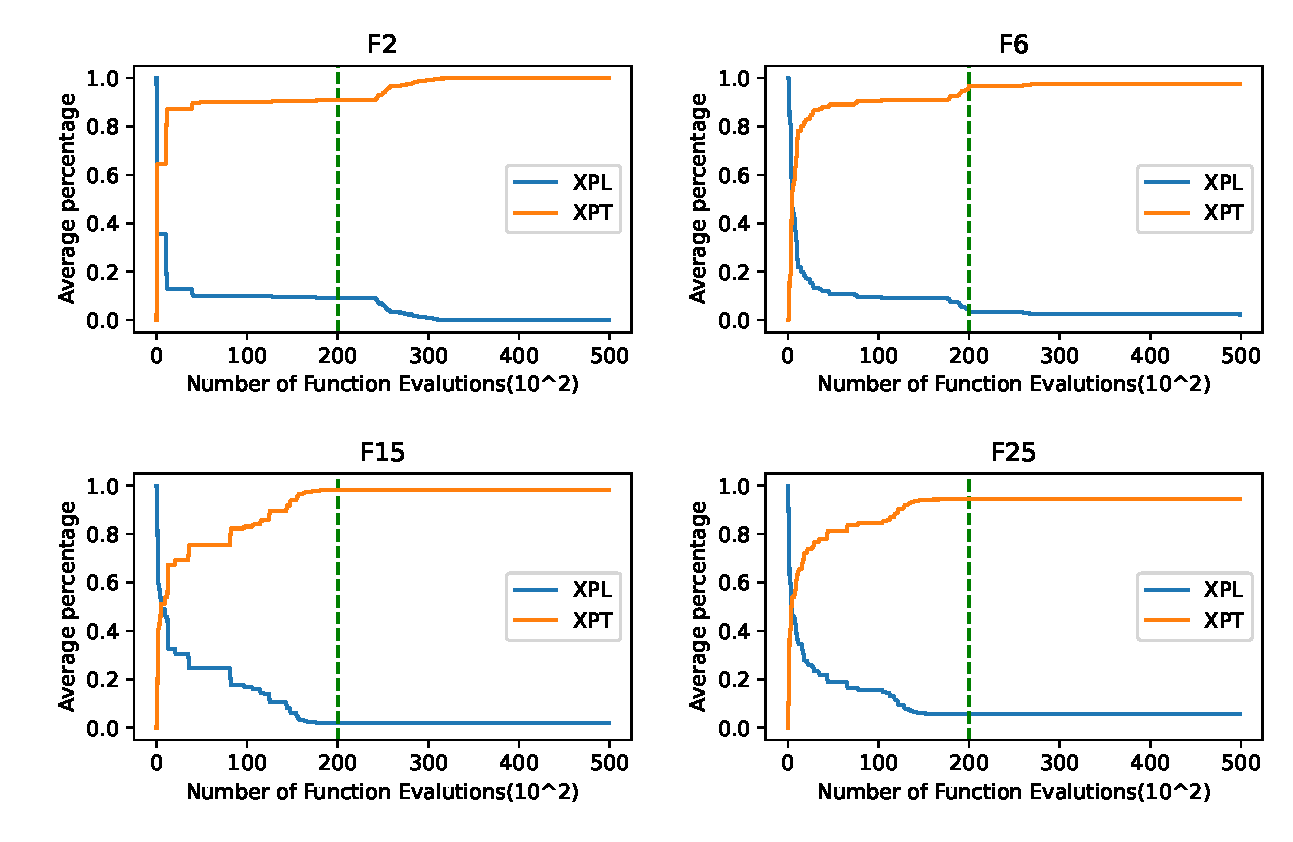
\includegraphics[width=0.9\columnwidth]{./explore.pdf}
 	\vspace{-4mm}
 	\caption{Exploration and exploitation percentage of DLES for F2, F6, F15, and F25 with 30 dimensions.}
 	\vspace{-4mm}
 	\label{explore}
 \end{figure}

Exploring and developing proportions within a population can reveal the current state of the population. In Fig.~\ref{explore}, we select representatives F2, F6, F15, and F25 to illustrate the population dynamics of DLES during the search process in the solution space on $D=30$. The dashed vertical line in the figure corresponds to  when DLES utilizes the network for reconstruction. The left side of the dashed line represents the exploration and sampling phase of our proposed DLES, while the right side represents the subsequent development phase. As the population state remains nearly constant during the subsequent development process, only the population state at the first 50,000 evaluations is displayed.

From Fig.~\ref{explore}, it is evident that when DLES employs the network for simulating the solution space, XPL's value approaches 0, XPT one approaches 1. The population has almost entirely transitioned to the development phase, signifying the conclusion of the exploration process. The data provided to train the network for reconstruction corresponds to the population's exploration path in the solution space, aligning precisely with the original intent of our algorithm design.

\textcolor{blue}{
The quantity and quality of training samples are crucial for effective network learning; hence, ensuring high-quality adequate training sample is of paramount importance. In terms of sample quantity, the quantity is controlled by the optimal exploration sampling count $T$. Theoretically, increasing the sampling iterations deepens the understanding of the solution space. A higher $T$ value results in more training samples, which enhances the network's performance. However, due to the limited number of evaluations, excessive allocation of evaluations to the exploration phase can lead to insufficient evaluations for subsequent algorithm exploitation. Therefore, a careful balance of $T$ is required. Table~\ref{Hyperparameters} discusses the impact of various $T$. It can be observed that, with consistent network training parameters, the algorithm achieves the best overall performance when $T$ is euqal to 100. If the sampling iterations are too few, the network struggles to learn effectively; if too many, it adversely affects the subsequent exploitation phase of the algorithm.}

\textcolor{blue}{
Regarding sample quality, we indirectly ensure the quality of training samples by measuring the exploration-exploitation ratio of the population. When $T$ is equal to 100, the evaluations consumed amount to 2000. As shown in Fig.~\ref{explore}, the population stabilizes at the same level, primarily remaining in the exploitation phase, indicating that the algorithm has largely completed its exploration phase. This stability ensures the quality of our training samples.
}

\subsection{Complexity Analysis}
DLES does not entail supplementary evaluation costs in its utilization of the network for learning and fitting. Consequently, it avoids incurring additional expenses in situations where constraints exist on the number of evaluations, rendering it particularly advantageous for problems characterized by limited evaluation resources.

In terms of space complexity, DLES differs from other algorithms as it necessitates additional storage for the dataset used in network training. However, the proportion of this data relative to the overall evaluation dataset is $1/K$, where $K$ is a parameter associated with the hyperparameter of the sampling iterations  $T$, the value of $1/K$ is exceptionally low at $0.0776$. Therefore, the increase in space complexity for DLES due to network augmentation does not exceed $O(N \cdot D)$. This implies that, in comparison to other algorithms, DLES does not exhibit a significant increase in overall space utilization.

The DLES's time complexity is closely tied to the training of the neural network. Specifically, the increased time is primarily consumed during the process of network training. The time consumption for network training is associated with the number of training epochs. The time complexity of the DLES algorithm is expressed as $O(n) = T \cdot O(N \cdot D) +  E \cdot \alpha \cdot T \cdot O(N \cdot D) + (G-T)\cdot O(N^{2} \cdot D)$, where $T$ is the number of updates to the population during the exploration process, $G$ is the total number of iterations, $E$ is the number of training epochs for the network, $\alpha \cdot T$ represents the number of iterations in each epoch and $\alpha$ belongs to the interval (0,1]. For our recommended parameter setting of the epoch is 10, the network increases time consumption does not exceed the $O(N \cdot D)$ range. It is essential to highlight that leveraging GPU acceleration during the neural network training process can further diminish the time required for training.

In Table~\ref{runtime}, we depict the time consumption for a single run on the CEC 2018 problem set under scenarios without network, with network training using CPU, and with network training using GPU. In Table~\ref{runtime}, we observe that the use of network training only increases the overall time consumption by approximately 14-18\%. However, it is noteworthy that the total time consumption with GPU acceleration is slightly higher than that with CPU usage. We hypothesize that this might be attributed to the time required for data transfer from CPU to GPU, particularly evident in scenarios with smaller problem dimensions and lesser data volume. In such cases, the data transfer process constitutes a significant portion of the overall time. As the problem dimensions increase, the proportion of time spent on data transfer gradually diminishes. The data in Table~\ref{runtime} largely aligns with our conjecture, in the case of $D$ = 100, the GPU training accelerates the process.

\begin{table}[!t]
	\centering
	\caption{Total runtime for a single execution on CEC 2018 across varying dimensions.}
	\vspace{-2mm}
	\label{runtime}
	%\phantom{0}
	\resizebox{\linewidth}{!}{
		\begin{tabular}{l|cccc|cc}
			\hline
			    & $D$ = 10 & $D$ = 30 & $D$ = 50 & $D$ = 100 & Total time & Growth rate \\
			\hline 
			NO Net & 44.0648  & 315.8045 & 630.8677 & \textbf{2522.8911} & 3513.6281 & 	-  \\
		    IN CPU & 85.1327  & 417.0270 & 752.5798 & \textbf{2761.5299} & 4016.2694 & 14.3\% \\
		    IN GPU & 157.7279 & 484.6854 & 784.5067 & \textbf{2729.6929} & 4156.6139 & 18.2\% \\
		    \hline    
		\end{tabular}
	}
\vspace{-2mm}
\end{table}
In summary, DLES excels in complexity analysis, circumventing additional evaluation costs, ensuring effective space utilization, and enabling GPU acceleration for high-dimensional problems.

\textcolor{blue}{
\subsection{Visualization of Reconstructed Exploration Path}
\begin{figure}[t]
	\centering
	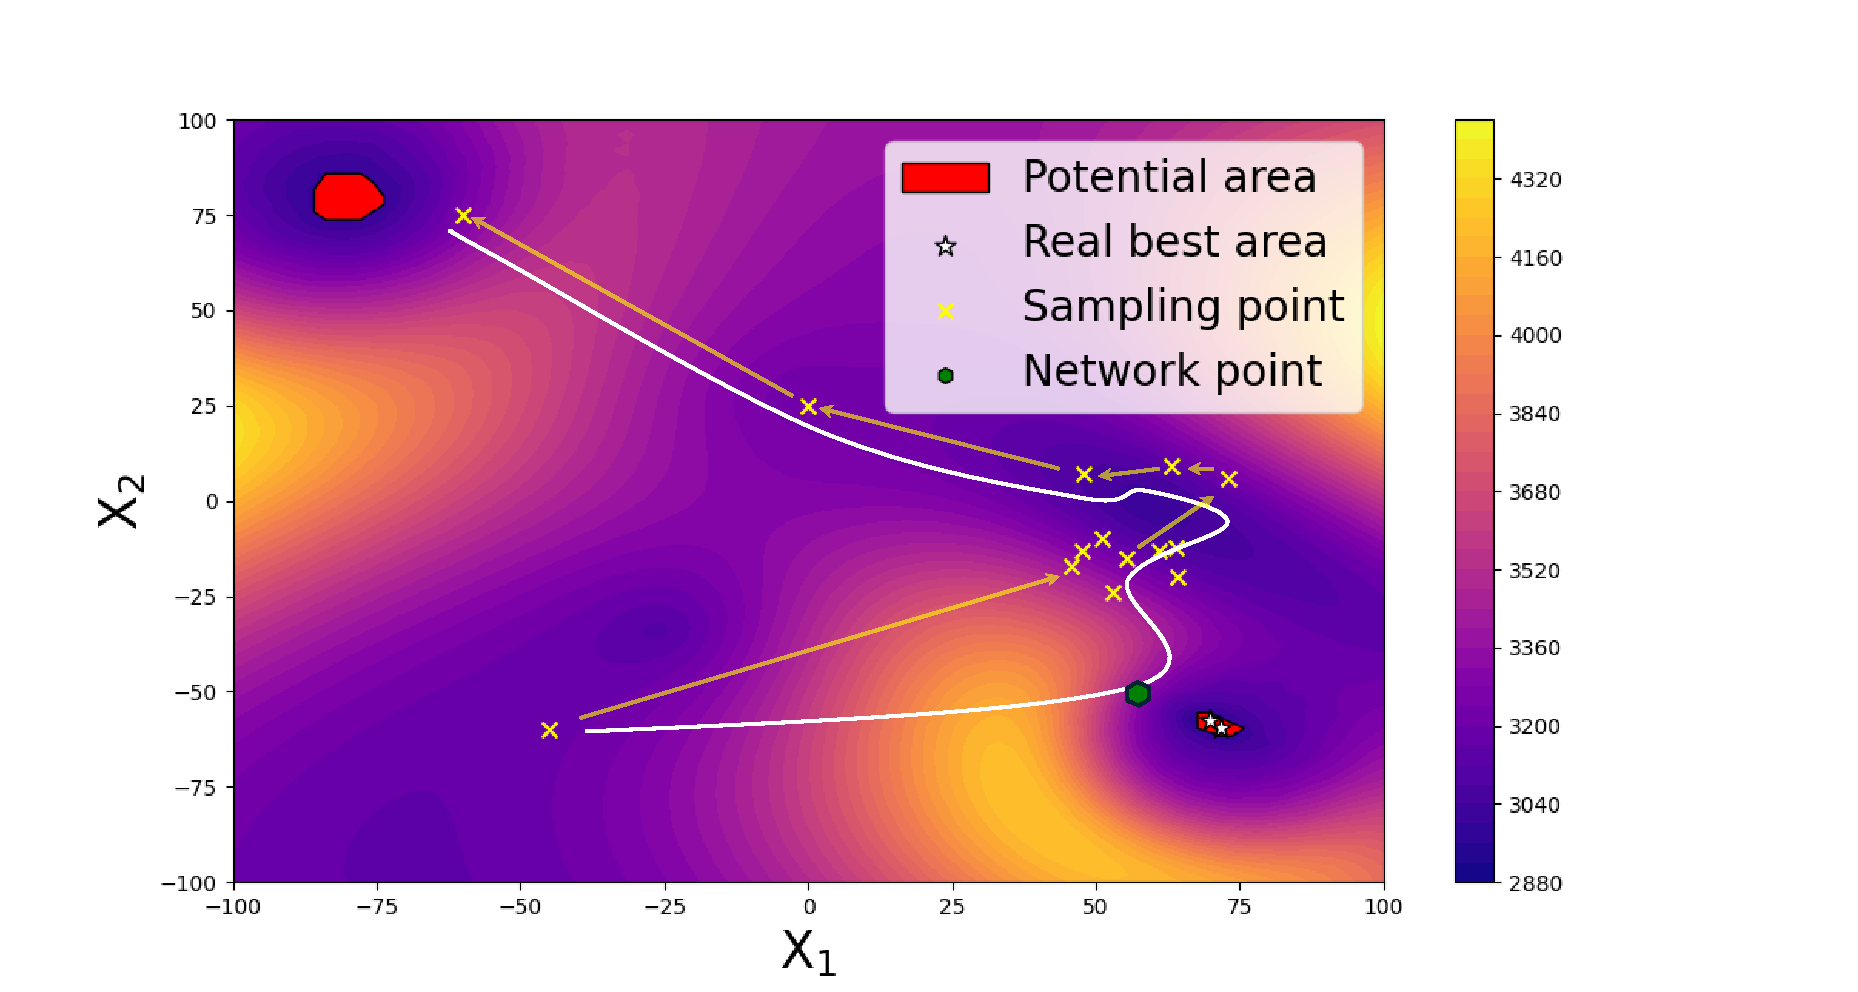
\includegraphics[width=1 \columnwidth]{./path.pdf}
	\vspace{-4mm}
	\caption{\textcolor{blue}{Visualization of the exploration process of DLES algorithm on CEC 2018 F27.}}
	\vspace{-4mm}
	\label{path}
\end{figure}
To better demonstrate the process and advantages of our proposed algorithm in reconstructing the solution space. We provide a two-dimensional visualization of the DLES algorithm's exploration process on CEC 2018 F27. As illustrated in Fig.~\ref{path}, the red regions represent potential areas, while the white pentagrams denote the true optimal points. The yellow crosses indicate the sampling locations during the algorithm's exploration within the search space. The green hexagons show the positions of the solutions with higher potential provided after network reconstruction. The colors in the figure represent the fitness values, with darker colors indicating smaller fitness values. For the F27 problem, the optimal fitness value is 2800.}

\textcolor{blue}{
The figure illustrates the sampling process of the algorithm as it explores the solution space. It is evident that the results of multiple samplings form an exploration path through the solution space. This path is indicated by yellow arrows connecting consecutive sampling points. The white curve represents the exploration path reconstructed by the network based on historical sampling points.}

\textcolor{blue}{
The visualization reveals that the algorithm is misled and gradually converges towards a local optimum. However, the network's reconstruction of the solution space corrected this issue, allowing the algorithm to subsequently explore and ultimately find the true optimal solution.}

\section{Conclusion}\label{sec_conclusion}
%In this paper, we propose a deep learning-based search space reconstruction evolution strategy algorithm (DLES) for reconstructing the authentic solution space. The algorithm utilizes a neural network to reconstruct exploration paths based on the sampling results of evolutionary operators in the solution space. In this way, the neural network can identify individuals with higher potential along the current exploration path, guiding subsequent developments using a hybrid sampling approach. Compared to traditional evolutionary operator sampling methods, the network reconstruction approach comprehensively understands the solution space, avoiding the complexity of high-dimensional solution spaces leading to local optima. Thus, our DLES algorithm can more effectively explore the solution space and discover more promising solutions.

%To evaluate the performance of DLES, we compare it with state-of-the-art champion algorithms. On benchmark test sets CEC 2014, CEC 2018, and CEC 2022, DLES demonstrates superior performance. When discussing the structure and hyperparameters of DLES, experiments show that DLES is insensitive to hyperparameters, exhibiting strong stability and generalization. We further analyze the population state during the DLES process and illustrate the impact of network reconstruction. This compelling evidence confirms that our proposed DLES can provide more development potential solutions. Finally, we conduct a preliminary analysis of the complexity of DLES. Analysis indicates that the increase in time and space complexity introduced by network reconstruction in the solution space is relatively low. Additionally, this process does not require extra evaluation counts.

\textcolor{blue}{
In this paper, we propose a deep learning-based search space reconstruction evolution strategy algorithm (DLES) for reconstructing the authentic solution space. The algorithm leverages a neural network to model exploration paths derived from the sampling results of evolutionary operators within the solution space. By doing so, the network identifies individuals with greater potential along the exploration path, guiding further search through a hybrid sampling approach. Unlike traditional evolutionary operator sampling methods, this network-based reconstruction offers a deeper understanding of the solution space, reducing the risk of local optima in high-dimensional problems. As a result, DLES more efficiently explores the solution space, uncovering promising solutions. To assess DLES's performance, we compare it to top algorithms on CEC and BBOB benchmarks, where it shows superior results. Experiments reveal that DLES is robust to hyperparameter changes, maintaining strong stability and generalization. We also examine the population state and the effects of network reconstruction, confirming DLES’s ability to find more promising solutions. Finally, we analyze DLES's complexity, showing that the added time and space costs from network reconstruction are minimal, with no extra evaluation counts needed.}

\textcolor{blue}{
DLES gathers crucial insights from the entire search process by fitting exploration paths. While modeling solution spaces by using neural networks is not new, previous methods often perform poorly because they attempt to fit the entire solution space, which results in excessive network complexity. By focusing solely on modeling exploration paths, we significantly reduce the network's load, allowing even simpler architectures to handle complex tasks. The incorporation of neural networks, with their powerful nonlinear fitting capabilities, enables DLES to combine the strengths of both network-driven and algorithm-driven approaches, highlighting the value of integrating deep learning with evolutionary algorithms in optimization challenges. }

In the future, we plan to extend the solution space reconstruction method to various aspects. Firstly, this paper primarily focuses on single-objective problems, and we hope to extend the DLES method to multi-objective problems. Secondly, by exploring and further developing more powerful evolutionary operators and strategies, we hope to enhance the potential of DLES. Finally, in this paper, we only reconstructed the exploratory part of the solution space. In the future, we will use more robust networks to reconstruct the more true exploration space. These extensions will contribute to further advancing the development of the DLES algorithm, providing more possibilities for its practical applications in real-world problems.
\vspace{-4mm}
\bibliographystyle{IEEEtran}
\bibliography{mybibfile}
%\vspace{-12mm}
%
\begin{IEEEbiography}[{
\includegraphics[width=1in,height=1.25in,clip,keepaspectratio]{./graph/Yaotong Song.jpg}}]{Yaotong Song}
	received the B.S. degree from Beijing University of Civil Engineering and Architecture, Beijing, China. He is currently pursuing the M.E. degree from the University of Toyama, Toyama, Japan. His current interests include computational intelligence and neural networks for real-world applications.
\end{IEEEbiography}
\vspace{-10mm}
\begin{IEEEbiography}[{
\includegraphics[width=1in,height=1.25in,clip,keepaspectratio]{./graph/Kaiyu Wang.jpg}}]{Kaiyu Wang}
	received the B.S. degree from Southwest University, Chongqing, China, in 2018, and the M.E. degree from the University of Toyama, Toyama, Japan, in 2022, where he is currently pursuing the Ph.D. degree. His current interests include computational intelligence and neural networks for real-world applications.
\end{IEEEbiography}
\vspace{-10mm}
\begin{IEEEbiography}[{
\includegraphics[width=1in,height=1.25in,clip,keepaspectratio]{./graph/ZH_Zhan.jpg}}]{Zhi-Hui Zhan} 
	(Fellow, IEEE) received the Ph.D. degree in computer science from Sun Yat-Sen University, Guangzhou China, in 2013.
	He is currently a Changjiang Scholar Young Professor and Gifted Professor with the College of Artificial Intelligence, Nankai University, Tianjin, China. His current research interests include evolutionary computation, swarm intelligence, and their applications in real-world problems. He is currently an Associate Editor of IEEE Transactions on Evolutionary Computation.
\end{IEEEbiography}
\vspace{-10mm}
\begin{IEEEbiography}[{
\includegraphics[width=1in,height=1.25in,clip,keepaspectratio]{./graph/Zhenyu Lei.jpg}}]{Zhenyu Lei}
	received the Ph.D. degree in Science and Engineering from the University of Toyama, Toyama, Japan, in 2023. He is currently an Assistant Professor with the Faculty of Engineering, University of Toyama, Japan. His current research interests include evolutionary computation, machine learning, and neural network for real-world applications and optimization problems.
\end{IEEEbiography}
\vspace{-10mm}

\begin{IEEEbiography}[{
\includegraphics[width=1in,height=1.25in,clip,keepaspectratio]{./graph/Shangce Gao.jpg}}]{Shangce Gao}
	(Senior Member, IEEE) received his Ph.D. degree in Innovative Life Science from University of Toyama, Toyama, Japan in 2011. He is currently a Professor with the Faculty of Engineering, University of Toyama, Japan. His current research interests include nature-inspired technologies, machine learning, and neural networks for real-world applications. He serves as an Associate Editor for many international journals such as IEEE Transactions on Neural Networks and Learning Systems, and IEEE/CAA Journal of Automatica Sinica. 
\end{IEEEbiography}

\end{document}

